\subsection{Le capteur AD8232 \label{sec:capteurAD8232}}
Le module AD8232 assure la surveillance des impulsions cardiaque. Le kit apporte en plus 3 électrodes à placer sur le corp du patient. Ce module, dont le datasheet est disponible sur ce \href{https://www.analog.com/media/en/technical-documentation/data-sheets/ad8232.pdf}{lien} (voir Annexe \ref{Datasheet}), est caractérisé principalement par :
\begin{itemize}
  \item un filtre passe-haut à deux pôles pour éliminer les artefacts de mouvement et le potentiel de demi-cellule d'électrode
  \item un amplificateur opérationnel sans contrainte pour construire un filtre passe-bas à trois pôles éliminant les bruits suplémentaires
  \item température nominale de $[0;70]$ et de travail $[-40; 85]$
  \item alimentation faible de 3,3V
  \item il est conçu pour extraire, amplifier et filtrer les petits signaux bipotentiels en présence de conditions bruyantes.
\end{itemize}

\begin{figure}[H]
  \centering
  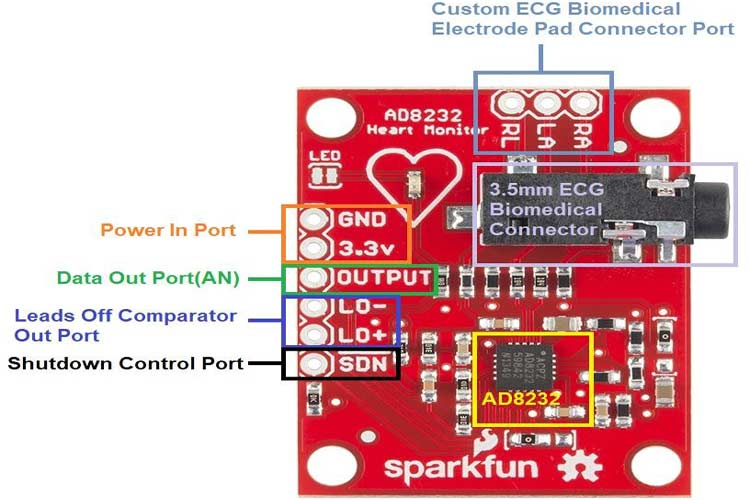
\includegraphics[scale=.4]{imgs/AD8232-Module-Overview.jpg}
  \caption{Description du capteur AD8232}
\end{figure}

Le tableau \ref{table:AD8232PINOUT} donne les pins du capteur
\begin{table}[H]
  \centering\small
  \begin{tabular}{lp{0.6\textwidth}}
  \toprule
  {\bf PIN}&{\bf Description}\\
  \toprule
  \mintinline{c++}{GND}&la masse\\
  \midrule
  \mintinline{c++}{3.3V}&alimentation\\
  \midrule
  \mintinline{c++}{Output} (ADC)&la sortie traitée du signal\\
  \midrule
  \mintinline{c++}{LO-}&leads off detection mode. \mintinline{c++}{LO-} est \mintinline{c++}{HIGH} si l'électrode rouge est déconnectée, et \mintinline{c++}{LOW} sinon\\
  \midrule
  \mintinline{c++}{LO+}&leads off detection mode. \mintinline{c++}{LO+} est \mintinline{c++}{HIGH} si l'électrode jaune est déconnectée, et \mintinline{c++}{LOW} sinon\\
  \midrule
  \mintinline{c++}{SDN}&Shutdown Control Input. Si cette pin est \mintinline{c++}{LOW}, le capteur active le mode de faible consommation\\
  \bottomrule
  \end{tabular}
  \caption{AD8232 PINOUT}
  \label{table:AD8232PINOUT}
\end{table}